\documentclass[11pt]{charter}

% El títulos de la memoria, se usa en la carátula y se puede usar el cualquier lugar del documento con el comando \ttitle
\titulo{People Behavior Tracking (PBT)} 

% Nombre del posgrado, se usa en la carátula y se puede usar el cualquier lugar del documento con el comando \degreename
%\posgrado{Carrera de Especialización en Sistemas Embebidos} 
%\posgrado{Carrera de Especialización en Internet de las Cosas} 
\posgrado{Carrera de Especialización en Inteligencia Artificial}
%\posgrado{Maestría en Sistemas Embebidos} 
%\posgrado{Maestría en Internet de las cosas}

% Tu nombre, se puede usar el cualquier lugar del documento con el comando \authorname
\autor{Hernán Contigiani} 

% El nombre del director y co-director, se puede usar el cualquier lugar del documento con el comando \supname y \cosupname y \pertesupname y \pertecosupname
\director{Urbano Pasquinel}
\pertenenciaDirector{Globant} 
% FIXME:NO IMPLEMENTADO EL CODIRECTOR ni su pertenencia
\codirector{} % si queda vacio no se deberíá incluir 
\pertenenciaCoDirector{}

% Nombre del cliente, quien va a aprobar los resultados del proyecto, se puede usar con el comando \clientename y \empclientename
\cliente{Technical Leader}
\empresaCliente{Globant}

% Nombre y pertenencia de los jurados, se pueden usar el cualquier lugar del documento con el comando \jurunoname, \jurdosname y \jurtresname y \perteunoname, \pertedosname y \pertetresname.
\juradoUno{Nombre y Apellido (1)}
\pertenenciaJurUno{pertenencia (1)} 
\juradoDos{Nombre y Apellido (2)}
\pertenenciaJurDos{pertenencia (2)}
\juradoTres{Nombre y Apellido (3)}
\pertenenciaJurTres{pertenencia (3)}
 
\fechaINICIO{5 de marzo de 2021}		%Fecha de inicio de la cursada de GdP \fechaInicioName
\fechaFINALPlanificacion{23 de abril de 2021} 	%Fecha de final de cursada de GdP
\fechaFINALTrabajo{agosto de 2021}		%Fecha de defensa pública del trabajo final


\begin{document}

\maketitle
\thispagestyle{empty}
\pagebreak


\thispagestyle{empty}
{\setlength{\parskip}{0pt}
\tableofcontents{}
}
\pagebreak


\section{Registros de cambios}
\label{sec:registro}


\begin{table}[ht]
\label{tab:registro}
\centering
\begin{tabularx}{\linewidth}{@{}|c|X|c|@{}}
\hline
\rowcolor[HTML]{C0C0C0} 
Revisión & {1}{c|}{\cellcolor[HTML]{C0C0C0}Detalles de los cambios realizados} & Fecha      \\ \hline
1.0      & Creación del documento                                          & 15/03/2021 \\ \hline
1.1      & Avances de la planificación & 17/03/2021 \\ \hline
1.2      & Modificaciones basadas en las devoluciones \newline
		   Historias de usuario											   & 22/03/2021 \\ \hline
1.3      & Modificaciones basadas en las devoluciones \newline
		   Gestión del tiempo y los requerimientos								   & 30/03/2021 \\ \hline
1.4      & Completar los últimos puntos de la planificación & 06/04/2021 \\ \hline
1.5      & Agregar fecha de finalización y corrección de typos & 11/04/2021 \\ \hline
%		   En varias líneas \newline
%		   A propósito                                                     %& dd/mm/aaaa \\ \hline
\end{tabularx}
\end{table}

\pagebreak



\section{Acta de constitución del proyecto}
\label{sec:acta}

\begin{flushright}
Buenos Aires, \fechaInicioName
\end{flushright}

\vspace{2cm}

Por medio de la presente se acuerda con el Ing. \authorname\hspace{1px} que su Trabajo Final de la \degreename\hspace{1px} se titulará ``\ttitle'', consistirá esencialmente en utilizar computer vision y deep learning para obtener información sobre el comportamiento de personas/clientes dentro de un recinto, y tendrá un presupuesto preliminar estimado de 748 hs de trabajo, con fecha de inicio \fechaInicioName\hspace{1px} y fecha de finalización \fechaFinalName.

Se adjunta a esta acta la planificación inicial.

\vfill

% Esta parte se construye sola con la información que hayan cargado en el preámbulo del documento y no debe modificarla
\begin{table}[ht]
\centering
\begin{tabular}{ccc}
\begin{tabular}[c]{@{}c@{}}Ariel Lutenberg \\ Director posgrado FIUBA\end{tabular} & \hspace{2cm} & \begin{tabular}[c]{@{}c@{}}\clientename \\ \empclientename \end{tabular} \vspace{2.5cm} \\ 
\multicolumn{3}{c}{\begin{tabular}[c]{@{}c@{}} \supname \\ Director del Trabajo Final\end{tabular}} \vspace{2.5cm} \\
%\begin{tabular}[c]{@{}c@{}}\jurunoname \\ Jurado del Trabajo Final\end{tabular}     &  & \begin{tabular}[c]{@{}c@{}}\jurdosname\\ Jurado del Trabajo Final\end{tabular}  \vspace{2.5cm}  \\
%\multicolumn{3}{c}{\begin{tabular}[c]{@{}c@{}} \jurtresname\\ Jurado del Trabajo Final\end{tabular}} \vspace{.5cm}                                                                     
\end{tabular}
\end{table}


\newpage

\section{Descripción técnica-conceptual del proyecto a realizar}
\label{sec:descripcion}

El sistema de monitoreo de comportamiento de personas (PBT) tiene como objetivo estudiar los movimientos que realiza una persona al ingresar a un espacio, a fin de obtener métricas sobre los lugares del local que visitó, cuánto tiempo permaneció en el recinto y si transitó por alguna zona de interés predefinida.

Para poder cumplir con el objetivo de estudiar el comportamiento de las personas dentro de un espacio es necesario poder detectar a las distintas personas, realizar un seguimiento de cada una y poder identificarlas aún cuando desaparecen del espacio de visión por unos segundos.

Para poder alcanzar el objetivo planteado se debe construir un pipeline de inteligencia artificial como se observa en la Figura \ref{fig:diagBloques}, el cual está comformado por un detector de personas, un tracker (seguidor) y un sistema que permita extraer características (embeddings) que luego el Engine utilizará para poder identificar personas que hayan salido del rango de visión por oclusiones o fuera de imagen.

\vspace{25px}

\begin{figure}[htpb]
\centering 
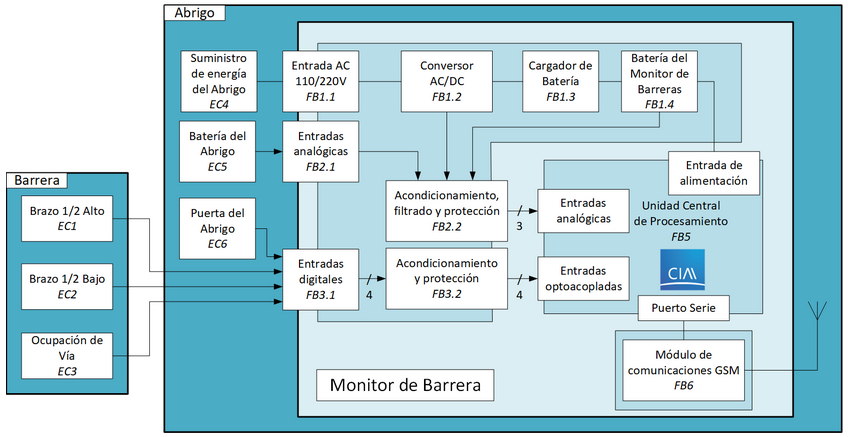
\includegraphics[width=.7\textwidth]{./Figuras/diagBloques.png}
\caption{Diagrama en bloques del sistema}
\label{fig:diagBloques}
\end{figure}

El objetivo principal del Engine es identificar a cada persona con un “id” único y analizar sus movimientos dentro del reciento, como también debe resolver las siguientes problemáticas:
\begin{itemize}
\item Resolver que una persona salga y entre del rango de visión, y en dicho caso, el sistema la debe identificar como la misma persona.
\item Resolver las oclusiones que puedan llegar a ocurrir (personas que tapan a otras personas en el rango de visión).
\item Mantener el id correcto entre las personas y evitar que los “id” se intercambien.
\end{itemize}

\newpage

Toda la información recolectada por el Engine será enviada a una aplicación web desarrollada en Python, la cual mostrará un dashboard con toda la información recolectada al momento. El Engine para poder realizar todo el labor mencionado necesita como entrada las personas detectadas en un video/imagen (la bounding box de cada una), un “id” tentativo entregado por el Tracker, y características (embeddings)  entregadas por un extractor. Para ello ya se estuvo trabajando y ensayando los siguientes modelos pre-entrenados:

\begin{itemize}
\item Detector: Se utilizará el modelo pre-entrenado “Yolo” como detector por excelencia para detectar personas en una imagen/video. Se utilizará la versión completa de Yolo, a fin de obtener la mayor precisión posible.
\item Tracker: Se utilizará el modelo pre-entrenado “DeepSort” como tracker por excelencia para asignar un primer “id” tentativo utilizando flujo óptimo, técnicas de seguimiento de patrones (Mean Shift) y un clasificador básico para resolver oclusiones momentáneas.
\item Extractor de características: Se ensayarán diferentes alternativas como extractor de atributos, extractor de vectores de personas, clasificadores de imágenes entrenados con datasets de personas, etc. Sea cual sea el modelo definitivo que se utilice, el objetivo es obtener un vector de características de cada persona detectada que permita al Engine identificar a las personas en el recinto.
\end{itemize}

\textbf{NOTA}: Las redes generadores de vectores (extractor) ya se encuentran pre entrenadas con datasets de personas y los modelos/pesos están disponibles en internet. Por una cuestión académica y reforzar este trabajo se realizará el entrenamiento fine-tuning de la red seleccionada como extractor, para luego comparar contra el modelo utilizado disponible en internet. Los datasets más utilizados para este propósito son el Market 1051 y DukeMTMC-reID.


\section{Identificación y análisis de los interesados}
\label{sec:interesados}

\begin{table}[ht]
%\caption{Identificación de los interesados}
%\label{tab:interesados}
\begin{tabularx}{\linewidth}{@{}|l|X|X|l|@{}}
\hline
\rowcolor[HTML]{C0C0C0} 
Rol           & Nombre y Apellido & Organización 	& Puesto 	\\ \hline
Auspiciante   & Empresa EEUU      & (confidencial) 	&        	\\ \hline
Cliente       & \clientename      &\empclientename	&        	\\ \hline
Impulsor      &                   &              	&        	\\ \hline
Responsable   & \authorname       & FIUBA        	& Alumno 	\\ \hline
Colaboradores &                   &              	&        	\\ \hline
Orientador    & \supname	      & \pertesupname 	& Director	Trabajo final \\ \hline
Equipo        & (confidencial) 	  & Globant         & IoT Engineer   	\\ \hline
Opositores    &                   &              	&        	\\ \hline
Usuario final &                   &              	&        	\\ \hline
\end{tabularx}
\end{table}

Nota: Por motivos de confidencialidad no puedo mencionar el nombre del auspiciante ni de los miembros del equipo.

\newpage

\section{1. Propósito del proyecto}
\label{sec:proposito}

El propósito de este proyecto es obtener métricas de los movimientos que realiza una persona al ingresar a un espacio, a fin de obtener los siguientes indicadores:
\begin{itemize}
\item Determinar cuántas personas se encuentran en el espacio de interés.
\item Determinar zonas de interés en el espacio y determinar cuántas y cuales personas transitaron por este. Las zonas de interés se dibujarán con polígonos en la imagen que representará al espacio de interés.
\item Determinar cuánto tiempo las personas estuvieron dentro del espacio y las diferentes zonas de interés.
\item Determinar cuando una persona abandona el espacio.
\end{itemize}

\section{2. Alcance del proyecto}
\label{sec:alcance}
Todas las pruebas se realizarán sobre videos (mp4) públicos, en donde haya un grupo de personas que permita su estudio de comportamiento. Se utilizarán videos que se acerquen lo mayor posible a un video que podría obtenerse de una cámara de seguridad de una tienda o un espacio. En caso de que la empresa consiga videos que puedan ayudar al problema, estos no podrán compartirse a menos que la empresa lo permita y en todo caso sólo se mostrarán los resultados o métricas alcanzadas en el dashboard. El dashboard \textbf{no mostrará el streaming de video} sino una representación del espacio y las métricas sobre el comportamiento de las personas monitoreadas.

Para la elaboración de este proyecto la parte del pipeline correspondiente al Detector + Tracker + Extractor se ejecutará en Colab. Se consumirá un video pregrabado mp4 el cual generará un archivo JSON con todos los datos recolectados del video que serán los inputs del Engine para que este luego los consuma finalizado este proceso. El Engine correrá en una máquina local o dispositivo dedicado utilizando como entrada el archivo de datos, y la aplicación web dashboard  en una máquina local o servicio en la nube conectada al Engine en real-time (a medida que el Engine consume el archivo y genera información, los resultados se verán reflejados en la App).

\begin{figure}[htpb]
\centering 
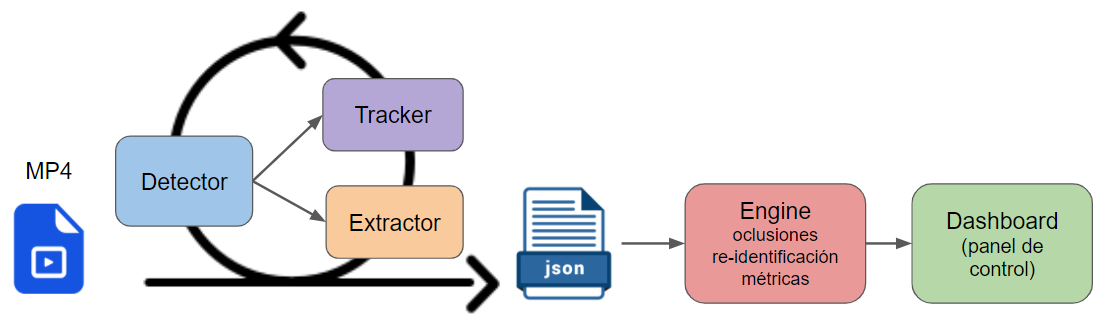
\includegraphics[width=.7\textwidth]{./Figuras/diagEjecucion.png}
\caption{Diagrama de ejecución del sistema}
\label{fig:diagEjecucion}
\end{figure}

\newpage

\section{3. Supuestos del proyecto}
\label{sec:supuestos}

Para el desarrollo del presente proyecto se supone que:

\begin{itemize}
\item Todo el proceso que requiera GPU será ejecutado en Colab (entorno virtual gratuito de Google para ejecutar modelos de IA).
\item Todo el proceso ejecutado en Colab no será real-time, la salida del sistema será un archivo que consuma luego el Engine.
\item En esta fase no se invertirá en hardware, se contará con Colab para el procesamiento pesado en GPU.
\item En esta etapa del proyecto no se realizará el deploy del sistema en ningún sistema embebido o servidor, se mantendrá todo en un entorno controlado de desarrollo (Colab + computadora personal).
\item Se utilizá diferentes videos que representen un escenario clásico de un local, tienda o recinto.
\item En esta fase no será requerido realizar corrección de imagen o deformación de los videos adquiridos, se buscaran videos sin deformaciones.
\item No se espera realizar el correcto seguimiento del 100\% de las personas, se establecerá un margen de aceptación para ello.
\item No se espera evitar problemas que surjan por movimientos o comportamientos de las personas que salgan de lo normal esperado.
\end{itemize}

\newpage

\section{4. Requerimientos}
\label{sec:requerimientos}

\begin{enumerate}
\item Grupo de requerimientos asociados con el pipeline de IA:
	\begin{enumerate}
	\item Detectar y seguir personas en un video, excluir otros elementos.
	\item Generar características que permitan luego re identificar personas perdidas.
	\item El sistema debe entregar como resultado un archivo con los datos de detección, seguimiento y características en formato JSON.
	\end{enumerate}
\item Grupo de requerimientos asociados con el Engine:
	\begin{enumerate}
	\item Consumir e interpretar los datos provenientes del pipeline de IA.
	\item Resolver problemáticas en el seguimiento de las personas utilizando sus características.
	\item Medir el comportamiento de cada persona con diferentes áreas de interés definidas en la aplicación.
	\item El sistema debe enviar los resultados en un JSON con toda la información de interés a ser consumida por la aplicación web.
	\end{enumerate}
\item Grupo de requerimientos asociados con la aplicación web:
\begin{enumerate}
	\item Mediante una interfaz web poder definir las zonas de interés en el espacio.
	\item Consumir e interpretar los datos provenientes del Engine.
	\item Se considerará que una persona es correctamente monitoreada si al menos se mantuvo su seguimiento el 80\% del tiempo que circuló en el recinto.
	\item Se considerará que el sistema funciona dentro de los parámetros aceptables si entre el 80\% y 100\% de las personas en el video fueron correctamente monitoreadas.
	\item Poder observar en tiempo real los datos que se obtienen de cada persona y las zonas definidas.
	\end{enumerate}
\item Grupo de requerimientos asociados con regulaciones:
\begin{enumerate}
	\item Los videos utilizados no inflijan derechos de privacidad.
	\item El sistema no asociará las personas en seguimiento con un persona física real.
	\item Las personas en seguimiento se harán referencia con un número incremental asociado a la base de datos, sin almacenar ningún tipo de información privada.
	\end{enumerate}
\end{enumerate}

\newpage

\section{Historias de usuarios (\textit{Product backlog})}
\label{sec:backlog}

Roles:
\begin{itemize}
\item Usuario - Quien utilizará el sistema desde la aplicación web. Consume los reportes del sistema y lo utiliza para mejorar el layout del reciento (podría ser el área de visuales de la tienda, el área de marketing o el área de diseño de ambientes).
\item Product Owner (PO) - El cliente y/o auspiciante del proyecto. Es aquel que vela por la realización del mismo y a su vez porta voz y visión del consumidor final del producto. El PO expone el avance del proyecto a su cartera de clientes a fin de posicionarlo en el mercado, por ello su preocupación e interés está muy enfocado en la experiencia de usuario, el proceso de puesta en marcha del producto en el local y  que el proyecto alcance las métricas establecidas a fin de utilizar dicha información como herramienta de negociación para conseguir más inversión.
\item Instalador - Quien instala el sistema en la tienda o reciento. El instalador es empleado y entrenado por el auspiciante del proyecto, se vale de la experiencia adquirida en otros productos similares y de las herramientas construidas que lo ayuden a la puesta en marcha del producto en el recinto.
\end{itemize}

Story points:
\begin{itemize}
\item Se realizarán 2 sprints por mes (sprints de 2 semanas).
\item Los sprints abarcan entre 40 y 50 horas de trabajo cada uno.
\item Se utilizará la escala de 1, 3, 5 y 8 puntos para las historias, siendo 8 puntos una historia que conlleva todo un sprint.
\begin{itemize}
\item Historias de 1 punto: Aquellas de bajo riesgo y rápida implementación principalmente asociadas con cambios cosméticos. Las historias asociadas con 1 punto se estiman que se resolverán en el día.
\item Historias de 3 puntos: Aquellas de bajo riesgo e implementación moderada principalmente asociadas con requerimientos de prioridad moderada. Las historias asociadas con 3 puntos se estiman que consumirán menos de la mitad de la capacidad de todo el sprint.
\item Historias de 5 puntos: Aquellas de riesgo moderado e implementación moderada principalmente asociadas con requerimientos de alta prioridad. Las historias asociadas con 5 puntos se estiman que consumirán la mitad de la capacidad de todo el sprint.
\item Historias de 8 puntos: Aquellas de riesgo alto e implementación compleja principalmente asociadas con requerimientos que requieren una investigación previa o de cuya implementación dependan otras tareas de alta prioridad. Las historias asociadas con 8 puntos se estiman que consumiran la capacidad de todo el sprint.
\end{itemize}
\end{itemize}

\newpage

Historias de usuario:
\begin{itemize}
\item Como PO, quiero detectar personas en un video, para poder monitorear su comportamiento. (8p)
\item Como PO, quiero re identificar a las personas ocluidas por otras, para mantener el monitoreo aún cuando la persona se pierde de vista por unos segundos. (8p)
\item Como PO, quiero conocer el accuracy de monitoreo y seguimiento, para conocer el estado de funcionamiento del sistema.
\item Como instalador, quiero una interfaz para dibujar las zonas de interés, para poder realizar el proceso de instalación más rápido. (8p)
\item Como instalador, quiero visualizar lo que está detectando el sistema, para poder verificar que la instalación se efectuó con éxito. (5p)
\item Como cliente, quiero poder visualizar el monitoreo de las personas en el recinto, para conocer como interactúan con el ambiente. (8p)
\item Como cliente, quiero un reporte diario de monitoreo, para conocer la cantidad de personas que ingresaron y el tiempo de permanencia en cada zona. (5p)
\item Como cliente, quiero un mapa de calor del recinto, para conocer las zonas en donde hubo mayor interacción. (3p)
\end{itemize}

\section{5. Entregables principales del proyecto}
\label{sec:entregables}

\begin{itemize}
\item Esquema del funcionamiento de cada pieza del pipeline de IA de Colab (código reservado para Globant).
\item Esquema del funcionamiento del Engine de seguimiento (código reservado para Globant).
\item Aplicación web para interactuar con el sistema y ejecutar los ensayos.
\item Informe final
\end{itemize}

\newpage

\section{6. Desglose del trabajo en tareas}
\label{sec:wbs}

\begin{enumerate}
\item Desarrollo del pipeline IA. (348hs)
	\begin{enumerate}
	\item Obtener y analizar videos. (48hs)
	\item Ensayo de modelos de detección y trackeo. (40hs)
	\item Ensayo del extractor de características DeepMAR. (40hs)
	\item Ensayo del extractor de características OsNet. (40hs)
	\item Integración del extractor de características en el pipeline de detección. (40hs)
	\item Ensayos de integración profunda del extractor con el tracker. (40hs)
	\item Integrar al pipeline un modelo para la predicción de poses de la persona. (20hs)
	\item Armar el dataset para el entrenamiento del modelo extractor con Tensorflow (TF). (30hs)
	\item Entrenar y ensayar el modelo extractor en TF. (30hs)
	\item Comparativas entre los modelos extractores entrenados con los modelos pre-entrenados obtenidos en la web. (20hs)	
	\end{enumerate}
\item Desarrollo del Engine de seguimiento. (160hs)
	\begin{enumerate}
	\item Desarrollo del sistema de clustering para la re identificación de personas. (40hs)
	\item Definir las zonas de interés a partir de un JSON o archivo. (20hs)
	\item Ubicar las personas en el plano relativo a la imagen, a fin de determinar su ubicación en el recinto (20hs)
	\item Realizar lógica de detección dentro de zonas. (20hs)
	\item Desarrollar las APIs para integrar el Engine con dashboard o aplicación web. (20hs)
	\item Mejorar el accuracy del sistema analizando casos de borde (40hs)
	\end{enumerate}
\item Desarrollo del dasboard/web app. (140hs)
	\begin{enumerate}
	\item Desarrollar la interfaz de usuario para definir las zonas de interés sobre una imagen (40hs)
	\item Desarrollar las APIs de comunicación con el Engine. (20hs)
	\item Desarrollar la interfaz de visualización de las métricas de las personas. (40hs)
	\item Desarrollar la interfaz de visualización de la representación de las personas en la tienda en tiempo real. (40hs)
	\end{enumerate}
\item Presentación del trabajo. (100hs)
	\begin{enumerate}
	\item Redacción del informe de avance. (20hs)
	\item Redacción de las memorias del proyecto. (60hs)
	\item Preparación de la presentación pública. (20hs)
	\end{enumerate}
\end{enumerate}

Cantidad total de horas: (748hs)

\newpage

\section{7. Diagrama de Activity On Node}
\label{sec:AoN}

En el la Figura \ref{fig:diagAoN} se ilustra el diagrama Activity On Node, la ruta crítica es resaltada en cuadros rojos. Aunque solo se cuenta con un recurso humano a lo largo del proyecto, se ejecutan tareas relacionadas en paralelo.
\begin{enumerate}
\item Las tareas están expresadas en horas.
\item La duración del camino crítico es de 380 horas.
\end{enumerate}

\begin{figure}[htpb]
\centering 
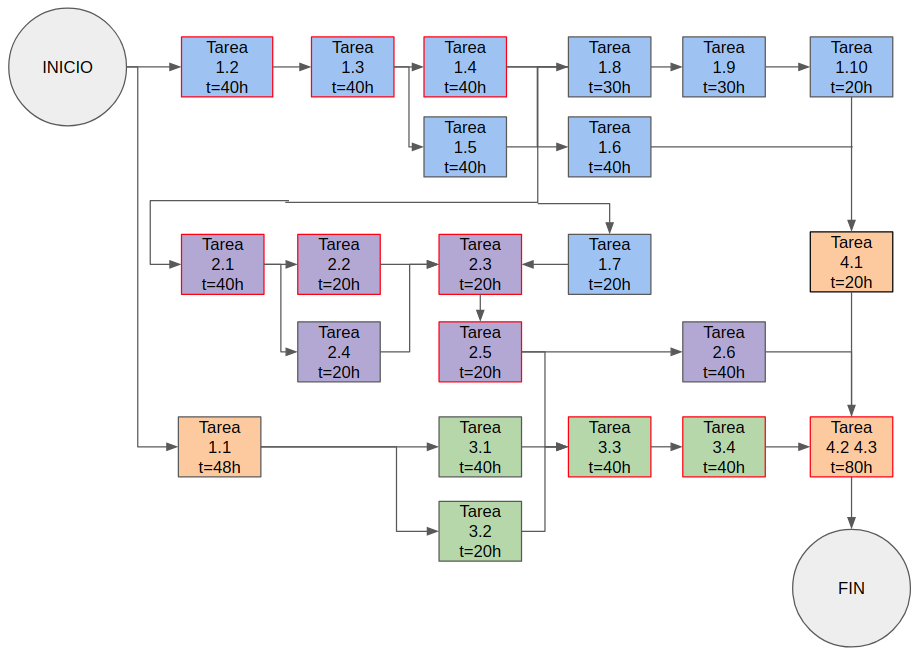
\includegraphics[width=1.\textwidth]{./Figuras/diagAoN.png}
\caption{Diagrama Activity On Node}
\label{fig:diagAoN}
\end{figure}

\newpage

\section{8. Diagrama de Gantt}
\label{sec:gantt}

En la Figura \ref{fig:ganttTable} y Figura \ref{fig:ganttTimeline} se ve el diagrama de gantt dividido en la tabla de tareas y la línea de tiempo.

\begin{figure}[htpb]
\centering 
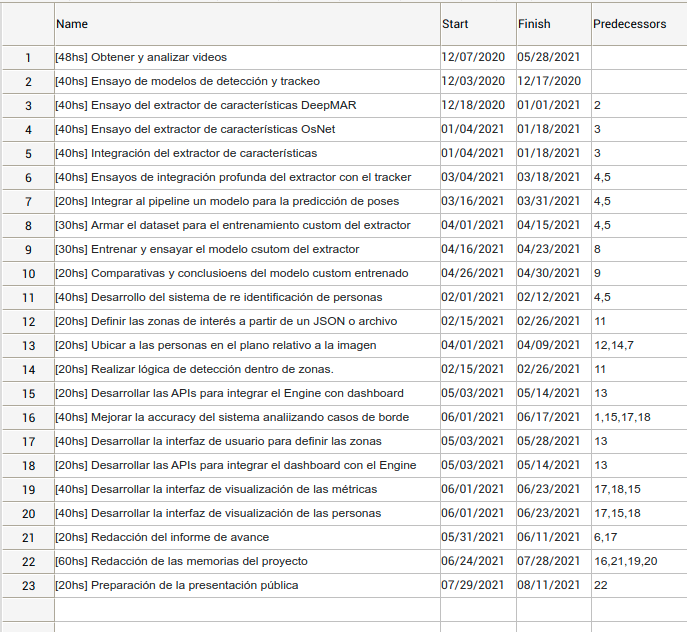
\includegraphics[width=1.\textwidth]{./Figuras/ganttTable.png}
\caption{Tabla de tareas Gantt}
\label{fig:ganttTable}
\end{figure}

\begin{figure}[htpb]
\centering 
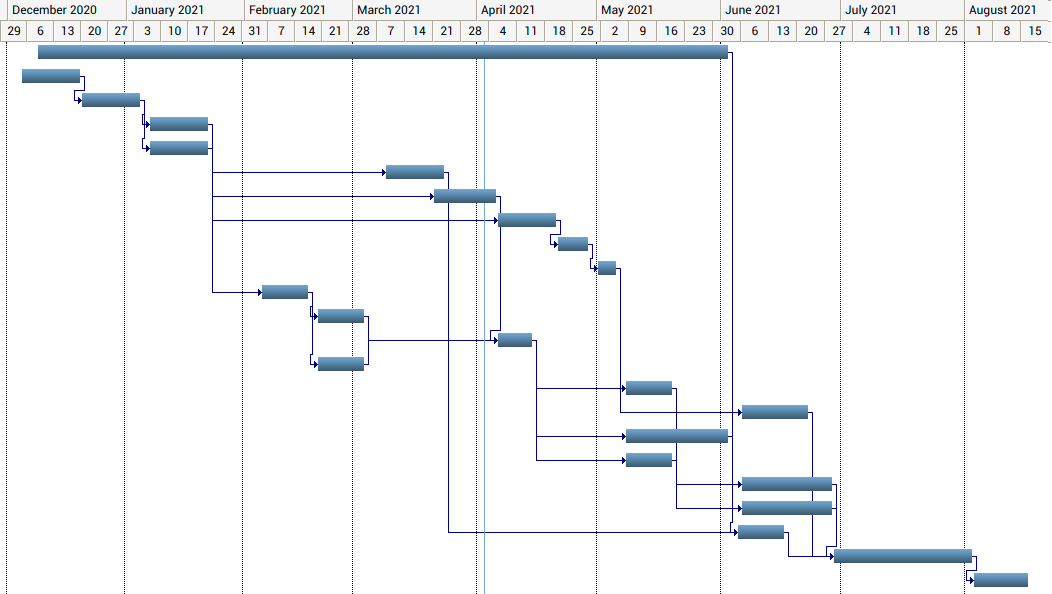
\includegraphics[width=1.\textwidth]{./Figuras/ganttTimeline.png}
\caption{Diagrama de Gantt}
\label{fig:ganttTimeline}
\end{figure}

\section{9. Matriz de uso de recursos de materiales}
\label{sec:recursos}


\begin{table}[htpb]
\label{tab:recursos}
\centering
\begin{tabularx}{\linewidth}{@{}|c|X|c|c|c|c|@{}}
\hline
\cellcolor[HTML]{C0C0C0} & \cellcolor[HTML]{C0C0C0} & \multicolumn{4}{c|}{\cellcolor[HTML]{C0C0C0}Recursos requeridos (horas)} \\ \cline{3-6} 
\multirow{-2}{*}{\cellcolor[HTML]{C0C0C0}\begin{tabular}[c]{@{}c@{}}Código\\ WBS\end{tabular}} & \multirow{-2}{*}{\cellcolor[HTML]{C0C0C0}\begin{tabular}[c]{@{}c@{}}Nombre de la tarea\end{tabular}} & Colab & PC & Youtube & Simulador \\ \hline
 1.1& Analizar videos y resultados	&  		&	&  30	& 18 \\ \hline
 1 	& Desarrollo Piepline IA 	&   300 &  		&  		&  \\ \hline
 2	& Desarrollo del Engine de seguimiento &  & 160  &  &  \\ \hline
 3	& Desarrollo del dashboard / web app & & 140 &  &  \\ \hline

\end{tabularx}%
\end{table}

*Simulador será cualquier programa o aplicación que permita obtener videos de muestra fuera de lo que es posible conseguir en canales como youtube, a fin de probar un escenario más cercano al layout de una tienda y poder generar videos más largos. Como posible simulador se podrá utilizar sistemas de renderizado 3D o juegos como el Sims.

\newpage

\section{10. Presupuesto detallado del proyecto}
\label{sec:presupuesto}

\begin{table}[htpb]
\centering
\begin{tabularx}{\linewidth}{@{}|X|c|r|r|@{}}
\hline
\rowcolor[HTML]{C0C0C0} 
\multicolumn{4}{|c|}{\cellcolor[HTML]{C0C0C0}COSTOS DIRECTOS} \\ \hline
\rowcolor[HTML]{C0C0C0} 
Descripción &
  \multicolumn{1}{c|}{\cellcolor[HTML]{C0C0C0}Cantidad} &
  \multicolumn{1}{c|}{\cellcolor[HTML]{C0C0C0}Valor unitario} &
  \multicolumn{1}{c|}{\cellcolor[HTML]{C0C0C0}Valor total} \\ \hline
Horas de ingeniería &
  \multicolumn{1}{c|}{648 horas} &
  \multicolumn{1}{c|}{\$6 USD} &
  \multicolumn{1}{c|}{\$3888 USD} \\ \hline
Computadora personal &
  \multicolumn{1}{c|}{1} &
  \multicolumn{1}{c|}{\$800 USD} &
  \multicolumn{1}{c|}{\$800 USD} \\ \hline
\multicolumn{1}{|l|}{} &
   &
   &
   \\ \hline
\multicolumn{1}{|l|}{} &
   &
   &
   \\ \hline
\multicolumn{3}{|c|}{SUBTOTAL} &
  \multicolumn{1}{c|}{\$4688 USD} \\ \hline
\rowcolor[HTML]{C0C0C0} 
\multicolumn{4}{|c|}{\cellcolor[HTML]{C0C0C0}COSTOS INDIRECTOS} \\ \hline
\rowcolor[HTML]{C0C0C0} 
Descripción &
  \multicolumn{1}{c|}{\cellcolor[HTML]{C0C0C0}Cantidad} &
  \multicolumn{1}{c|}{\cellcolor[HTML]{C0C0C0}Valor unitario} &
  \multicolumn{1}{c|}{\cellcolor[HTML]{C0C0C0}Valor total} \\ \hline
Licencia del sistema de gestión &
  \multicolumn{1}{c|}{1} &
  \multicolumn{1}{c|}{\$14 USD} &
  \multicolumn{1}{c|}{\$14 USD} \\ \hline
Costo de almacenamiento 100G &
  \multicolumn{1}{c|}{1} &
  \multicolumn{1}{c|}{\$20 USD} &
  \multicolumn{1}{c|}{\$20 USD} \\ \hline
\multicolumn{1}{|l|}{} &
   &
   &
   \\ \hline
\multicolumn{3}{|c|}{SUBTOTAL} &
  \multicolumn{1}{c|}{\$34 USD} \\ \hline
\rowcolor[HTML]{C0C0C0}
\multicolumn{3}{|c|}{TOTAL} & \$4722 USD
   \\ \hline
\end{tabularx}%
\end{table}


\section{11. Matriz de asignación de responsabilidades}
\label{sec:responsabilidades}

\begin{table}[htpb]
\centering
\resizebox{\textwidth}{!}{%
\begin{tabular}{|c|c|c|c|c|c|}
\hline
\rowcolor[HTML]{C0C0C0} 
\cellcolor[HTML]{C0C0C0} &
  \cellcolor[HTML]{C0C0C0} &
  \multicolumn{4}{c|}{\cellcolor[HTML]{C0C0C0}Listar todos los nombres y roles del proyecto} \\ \cline{3-6} 
\rowcolor[HTML]{C0C0C0} 
\cellcolor[HTML]{C0C0C0} &
  \cellcolor[HTML]{C0C0C0} &
  Responsable &
  Orientador &
  Equipo &
  Cliente \\ \cline{3-6} 
\rowcolor[HTML]{C0C0C0} 
\multirow{-3}{*}{\cellcolor[HTML]{C0C0C0}\begin{tabular}[c]{@{}c@{}}Código\\ WBS\end{tabular}} &
  \multirow{-3}{*}{\cellcolor[HTML]{C0C0C0}Nombre de la tarea} &
  \authorname &
  \supname &
  \clientename &
  Usuario \\ \hline
 1 & Desarrollo Piepline IA & P & A & I &  \\ \hline
 2 & Desarrollo del Engine & P & I & A &  \\ \hline
 3 & Desarrollo del dashboard & P & I & A & C \\ \hline
 4 & Presentación del trabajo & P & A & I &  \\ \hline
\end{tabular}%
}
\end{table}


Referencias:
\begin{itemize}
	\item P = Responsabilidad Primaria
	\item S = Responsabilidad Secundaria
	\item A = Aprobación
	\item I = Informado
	\item C = Consultado
\end{itemize}

\newpage

\section{12. Gestión de riesgos}
\label{sec:riesgos}

A lo largo del proyecto se hacen visibles los siguientes riesgos de los cuales se presenta una gestión
de los mismos.
 
Riesgo 1: No disponer del material en video necesario para validar todas las funcionalidades del sistema.
\begin{itemize}
\item Severidad (S): Este riesgo tiene una severidad alta porque se depende del material en video encontrado para poder validar el pipeline de IA y las funcionalidades que se describen en el proyecto. (10).
\item Probabilidad de ocurrencia (O): La probabilidad de este riesgo es alta porque es muy común en proyectos de inteligencia artificial que no se cuenten con tantos datos como los que se deseara. (8)
\end{itemize}   

Riesgo 2: No alcanzar las métricas pautadas para el sistema de seguimiento.
\begin{itemize}
\item Severidad (S): Este riesgo tiene una severidad alta porque uno de los factores más importantes del proyecto es la precisión de seguimiento. (8)
\item Ocurrencia (O): La probabilidad de este riesgo es baja porque antes de comenzar el proyecto se analizó de que fuera factible alcanzar las métricas pautadas, y en caso de existir una limitación por el layout del local se acotará el área de monitoreo al área efectiva con mayor precisión. (4)
\end{itemize}

Riesgo 3: No poder re identificar aquellas personas que al salir y entrar en cámara cambian su apariencia o vestimenta.
\begin{itemize}
\item Severidad (S): Este riesgo tiene una severidad baja porque parte del margen del sistema contempla estos casos de borde (4).
\item Ocurrencia (O): La probabilidad de este riesgo es muy baja porque justo se tiene que dar el caso de que la persona cambie su apariencia fuera de cámara, Mientras la persona esté en el área de visión, el tracker mantendrá el correcto seguimiento a pesar de cambiar su apariencia. (2)
\end{itemize}

Riesgo 4: No sea posible entrenar el modelo OsNet en Colab.
\begin{itemize}
\item Severidad (S): Este riesgo tiene una severidad muy baja porque el entrenamiento del modelo OsNet es unicamente con fin académico. (2)
\item Ocurrencia (O): La probabilidad de este riesgo es alta porque los recursos de Colab son limitados. (10)
\end{itemize}

\newpage

Riesgo 5: No cumplir con las fechas estimadas de desarrollo del proyecto.
\begin{itemize}
\item Severidad (S): Este riesgo tiene una severidad alta porque los recursos dedicados a este proyecto tienen futuras asignaciones concluida esta etapa. (8)
\item Ocurrencia (O): La probabilidad de este riesgo es baja porque hasta el momento el proyecto cumplió con todas las fechas importantes. (4)
\end{itemize}


b) Tabla de gestión de riesgos:      (El RPN se calcula como RPN=SxO)

\begin{table}[htpb]
\centering
\begin{tabularx}{\linewidth}{@{}|X|c|c|c|c|c|c|@{}}
\hline
\rowcolor[HTML]{C0C0C0} 
Riesgo & S & O & RPN & S* & O* & RPN* \\ \hline
   No disponer del material en video necesario    & 10  & 8   &  80   &  10  &  2  &  20    \\ \hline
   No alcanzar las métricas pautadas para el sistema de seguimiento    &  8  & 4   &  32   &  8  &   3 &   24   \\ \hline
   No poder re identificar personas que cambian de apariencia    &  4  & 2   &   8  &   - &  -  &  -    \\ \hline
   No sea posible entrenar el modelo OsNet en Colab    &  2  & 10  &  20   &  -  & -   &  -    \\ \hline
   No cumplir con las fechas estimadas    &  8  & 4   &  32   &  8  & 2   &  16    \\ \hline
\end{tabularx}%
\end{table}

Criterio adoptado: 
Se tomarán medidas de mitigación en los riesgos cuyos números de RPN sean mayores a 30.

Nota: los valores marcados con (*) en la tabla corresponden luego de haber aplicado la mitigación.

c) Plan de mitigación de los riesgos que originalmente excedían el RPN máximo establecido:

Riesgo 1: Como plan de mitigación se utilizarán simuladores o programas de renderizado 3D para poner a prueba todas las funcionalidades del sistema.
\begin{itemize}
\item Severidad (S): La severidad de este riesgo sigue siendo la misma. (10).
\item Probabilidad de ocurrencia (O): La probabilidad de este riesgo baja bastante, porque aquello que no pueda ser evaluado con videos reales se llevará a prueba en modelos de renderizado y entornos controlados. (2)
\end{itemize}

Riesgo 2: Como plan de mitigación está planificada una historia de usuario para contemplar los casos de borde en el sistema y así aumentar la precisión lo más posible.
\begin{itemize}
\item Severidad (S): La severidad de este riesgo sigue siendo la misma. (8).
\item Probabilidad de ocurrencia (O): La probabilidad de este riesgo baja muy poco ya que estamos hablando de un trabajo fino, pero se reduce lo suficiente para alcanzar las métricas deseadas. (3)
\end{itemize}

Riesgo 5: Como plan de mitigación se realizarán reuniones semanales atacar cualquier problema o improvisto a tiempo.
\begin{itemize}
\item Severidad (S): La severidad de este riesgo sigue siendo la misma. (8).
\item Probabilidad de ocurrencia (O): La probabilidad de este riesgo baja ya que se llevará un control semanal del avance del proyecto. (2)
\end{itemize}
 
\newpage
 
\section{13. Gestión de la calidad}
\label{sec:calidad}

\begin{itemize} 
\item Req \#1.1: Detectar y seguir personas en un video, excluir otros elementos.
\begin{itemize}
\item Verificación: consumir un video y verificar visualmente que solamente sean detectadas personas. 
\item Validación: Realizar un video post procesado de salida que verifique que solo son detectadas personas en el video.  
\end{itemize}
\end{itemize}

\begin{itemize} 
\item Req \#1.2: Generar características que permitan luego re identificar personas perdidas.
\begin{itemize}
\item Verificación: Ensayar los diferentes extractores de características propuestos y medir cual de ellos arroja mejores métricas de características. Con dicho extractor calcular si la distancia entre vectores que caracterizan a diferentes personas es mayor a la distancia entre vectores que pertenecen a una misma persona (evaluar que tan diferentes son los vectores de distintas personas vs los vectores de una misma persona).
\item Validación: Realizar un video en donde se vea como el sistema identifica a cada persona en el video utilizando unicamente los vectores obtenidos de estas.
\end{itemize}
\end{itemize}

\begin{itemize} 
\item Req \#1.3 y Req \#2.1: El sistema debe entregar como resultado un archivo con los datos de detección, seguimiento y características en formato JSON y ser consumido por el Engine.
\begin{itemize}
\item Verificación: Exportar en un archivo JSON la salida del pipeline de IA con los datos de detección, seguimiento y características para luego consumir dicho archivo con el Engine y validar que encuentra correctamente a las personas en el video.
\item Validación: Realizar un video en donde se vea la salida obtenida desde el Engine, validando la detección y el seguimiento de las personas en le video.
\end{itemize}
\end{itemize}

\begin{itemize} 
\item Req \#2.3: Medir el comportamiento de cada persona con diferentes áreas de interés definidas en la aplicación.
\begin{itemize}
\item Verificación: Observar los logs de la consola y verificar que la persona fue efectivamente detectada dentro de cada zona definida.
\item Validación: Realizar un video en donde la caja que representa a cada persona se pinte del color de cada zona al ingresar a esta.
\end{itemize}
\end{itemize}

\begin{itemize} 
\item Req \#3.3: Se considerará que una persona es correctamente monitoreada si al menos se mantuvo su seguimiento el 80\% del tiempo que circulo en el recinto.
\begin{itemize}
\item Verificación: Observar los logs de las métricas de cada persona y verificar el cumplimiento de dicha métrica.
\item Validación: Realizar un gráfico con el porcentaje de detección de cada persona y verificar el cumplimiento de dicha métrica.
\end{itemize}
\end{itemize}

\newpage

\begin{itemize} 
\item Req \#3.4: Se considerará que el sistema funciona dentro de los parámetros aceptables si entre el 80\% y el 100\% de las personas en el video fueron correctamente monitoreadas.
\begin{itemize}
\item Verificación: Observar los logs de las métricas de cada persona y verificar el cumplimiento de dicha métrica.
\item Validación: Realizar un gráfico con el porcentaje de detección de cada persona y verificar el cumplimiento de dicha métrica.
\end{itemize}
\end{itemize}

\begin{itemize} 
\item Req \#4.2 y Req \#4.3: El sistema no asociará a las personas en el video con una persona física, se hará referencia a las mismas con un número incremental asociado a la base de datos.
\begin{itemize}
\item Verificación: Observar la base de datos con todos los IDs generados.
\item Validación: Visualizar en la interfaz de la aplicación el seguimiento de las personas por números.
\end{itemize}
\end{itemize}

\newpage

\section{14. Comunicación del proyecto}
\label{sec:comunicaciones}

El plan de comunicación del proyecto es el siguiente:

\begin{table}[htpb]
\centering
\begin{tabularx}{\linewidth}{@{}|X|C{2.4cm}|C{3cm}|C{1.8cm}|C{2cm}|C{2.1cm}|@{}}
\hline
\rowcolor[HTML]{C0C0C0} 
\multicolumn{6}{|c|}{\cellcolor[HTML]{C0C0C0}PLAN DE COMUNICACIÓN DEL PROYECTO}           \\ \hline
\rowcolor[HTML]{C0C0C0} 
¿Qué comunicar? & Audiencia & Propósito & Frecuencia & Método de comunicac. & Responsable \\ \hline
 Avances de Plan de trabajo    &  Clase Gestión de Proyectos & Evitar errores y recibir feedback & Semanal  &  Correo y formulario                    &  \authorname            \\ \hline
  Avances del proyecto  &   \clientename        &  Avance semanal          &   Semanal   &   Video llamada  &    \authorname          \\ \hline
  Avances de validación y verificación & Director de proyecto          &  Avance y resultados         &   Mensual         &   Video llamada                   &       \authorname       \\ \hline
  Presentación final del proyecto              &   Jurados y Director        &  Definición y puesta en común         &  Única vez          &            Presentación y memorias del proyecto          &   \authorname          \\ \hline
\end{tabularx}
\end{table}

\section{15. Gestión de compras}
\label{sec:compras}

No es requerido realizar ningún tipo de compra para este proyecto.

\newpage

\section{16. Seguimiento y control}
\label{sec:seguimiento}

\begin{longtable}{|m{1cm}|m{3.5cm}|m{2.2cm}|m{2cm}|m{3cm}|m{1.5cm}|}
\hline
\rowcolor[HTML]{C0C0C0} 
\multicolumn{6}{|c|}{\cellcolor[HTML]{C0C0C0}SEGUIMIENTO DE AVANCE}                                                                       \\ \hline
\rowcolor[HTML]{C0C0C0} 
Tarea del WBS 			& Indicador de avance & Frecuencia de reporte & Resp. de seguimiento & Persona a ser informada & Método de comunic. \\ \hline
\endfirsthead

\hline
\rowcolor[HTML]{C0C0C0} 
\multicolumn{6}{c}{\cellcolor[HTML]{C0C0C0}SEGUIMIENTO DE AVANCE}                                                                       \\ \hline
\rowcolor[HTML]{C0C0C0} 
Tarea del WBS 			& Indicador de avance & Frecuencia de reporte & Resp. de seguimiento & Persona a ser informada & Método de comunic. \\ \hline
\endhead

\multicolumn{6}{c}{Continúa}
\endfoot

\endlastfoot

1	& Pipeline IA completo al 54\%, pendiente entrenamiento de OsNet y obtener videos simulados  & Semanal & \authorname & \clientename, \supname & email \\ \hline
2	& Engine completo al 50\%, pendiente el desarrollo de APIs para integrar con la app web y analizar casos de borde & Semanal & \authorname & \clientename, \supname & email \\ \hline
3	& El desarrollo de la applicación web no ha comenzado (0\%) & Mensual & \authorname & \clientename, \supname & email \\ \hline
4	& Presentación del trabajo final (0\%) & Mensual & \authorname & \clientename, \supname & email \\ \hline

\end{longtable}

\section{17. Procesos de cierre}    
\label{sec:cierre}

A continuación se describen las pautas que darán cierre al proyecto:

\begin{itemize}
\item Reunión por video llamada con el director y el líder del proyecto a fin de analizar las conclusiones del proyecto, retrospectiva y revisión para futuros trabajos.
\item Presentación y demostración del proyecto ante jurados mediante diapositivas y/o vídeos.
\end{itemize}


\end{document}
